\DTLloaddb[]{factors}{data/factors_influence.csv}

\newpage
\section{Influência dos fatores}

Para cada análise foi calculada a influência individual de cada fator e a influência conjunta. Também, foram gerados os gráficos de efeito principal, onde pode-se comparar os níveis de um mesmo fator, desconsiderando o outro fator, e de interação, onde, dado um nível de um fator, pode-se comparar sua interação com os níveis do outro fator.


\subsection{Análise 1}

\begin{table}[H]
\centering
\begin{tabular}{|c|c|}
    \hline \textbf{Fator} & \textbf{Influência} \\ 
    \hline Alocação & \DTLfetch{factors}{Answer variable}{L1-dcache-loads}{Alocation influence} \\
    \hline Otimização & \DTLfetch{factors}{Answer variable}{L1-dcache-loads}{Optimization influence} \\
    \hline Combinada & \DTLfetch{factors}{Answer variable}{L1-dcache-loads}{Combined influence} \\
    \hline
\end{tabular}
\end{table}


\begin{center}
  \makebox[\textwidth]{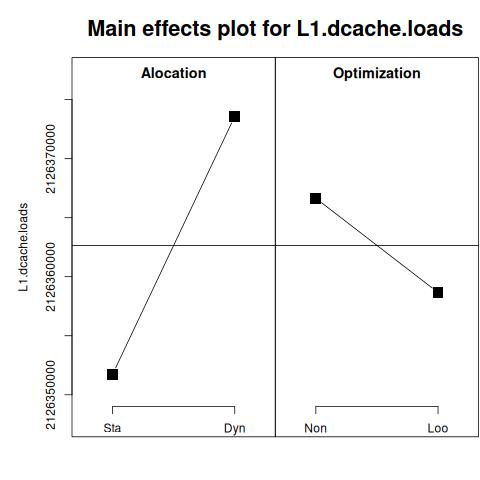
\includegraphics[width=0.6\textwidth]{data/plot/main-effects-cl.jpg}}
\end{center}
\begin{center}
  \makebox[\textwidth]{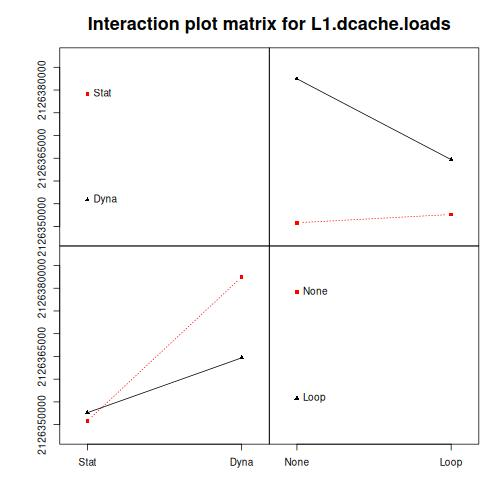
\includegraphics[width=0.6\textwidth]{data/plot/interaction-cl.jpg}}
\end{center}


\subsection{Análise 2}


\begin{table}[H]
\centering
\begin{tabular}{|c|c|}
    \hline \textbf{Fator} & \textbf{Influência} \\ 
    \hline Alocação & \DTLfetch{factors}{Answer variable}{L1-dcache-loads-misses}{Alocation influence} \\
    \hline Otimização & \DTLfetch{factors}{Answer variable}{L1-dcache-loads-misses}{Optimization influence} \\
    \hline Combinada & \DTLfetch{factors}{Answer variable}{L1-dcache-loads-misses}{Combined influence} \\
    \hline
\end{tabular}
\end{table}

\begin{center}
  \makebox[\textwidth]{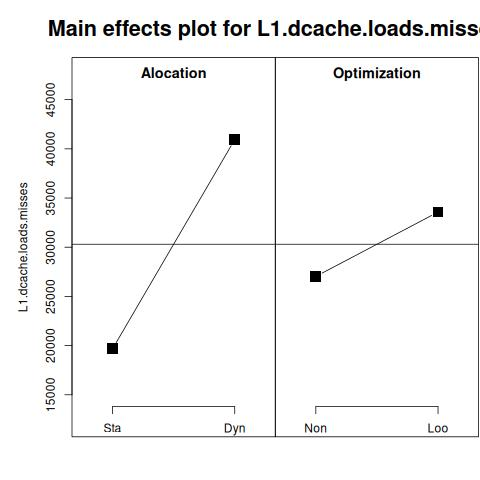
\includegraphics[width=0.6\textwidth]{data/plot/main-effects-clm.jpg}}
\end{center}
\begin{center}
  \makebox[\textwidth]{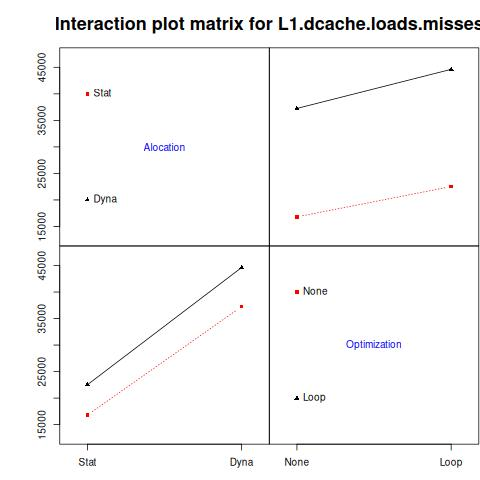
\includegraphics[width=0.6\textwidth]{data/plot/interaction-clm.jpg}}
\end{center}


\subsection{Análise 3}

A influência na variável \textit{branch-instructions} da alocação foi \DTLfetch{factors}{Answer variable}{branch-instructions}{Alocation influence}, da otimização foi \DTLfetch{factors}{Answer variable}{branch-instructions}{Optimization influence} e combinada foi \DTLfetch{factors}{Answer variable}{branch-instructions}{Combined influence}.

\begin{table}[H]
\centering
\begin{tabular}{|c|c|}
    \hline \textbf{Fator} & \textbf{Influência} \\ 
    \hline Alocação & \DTLfetch{factors}{Answer variable}{branch-instructions}{Alocation influence} \\
    \hline Otimização & \DTLfetch{factors}{Answer variable}{branch-instructions}{Optimization influence} \\
    \hline Combinada & \DTLfetch{factors}{Answer variable}{branch-instructions}{Combined influence} \\
    \hline
\end{tabular}
\end{table}

\begin{center}
  \makebox[\textwidth]{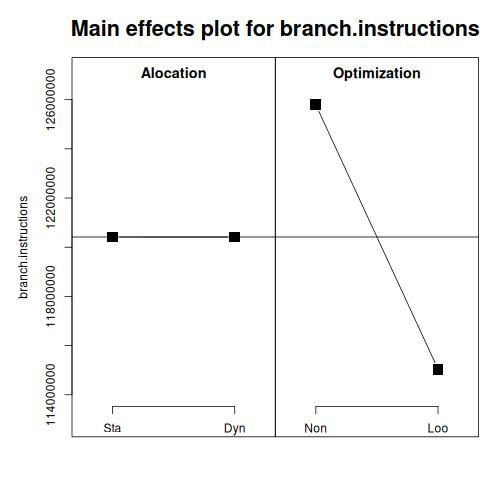
\includegraphics[width=0.6\textwidth]{data/plot/main-effects-bi.jpg}}
\end{center}
\begin{center}
  \makebox[\textwidth]{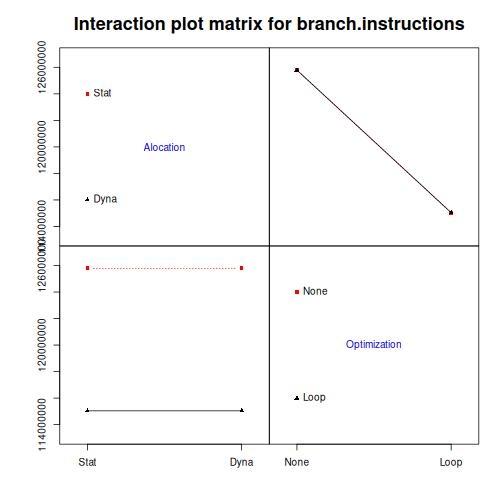
\includegraphics[width=0.6\textwidth]{data/plot/interaction-bi.jpg}}
\end{center}



\subsection{Análise 4}

\begin{table}[H]
\centering
\begin{tabular}{|c|c|}
    \hline \textbf{Fator} & \textbf{Influência} \\ 
    \hline Alocação & \DTLfetch{factors}{Answer variable}{branch-misses}{Alocation influence} \\
    \hline Otimização & \DTLfetch{factors}{Answer variable}{branch-misses}{Optimization influence} \\
    \hline Combinada & \DTLfetch{factors}{Answer variable}{branch-misses}{Combined influence} \\
    \hline
\end{tabular}
\end{table}

\begin{center}
  \makebox[\textwidth]{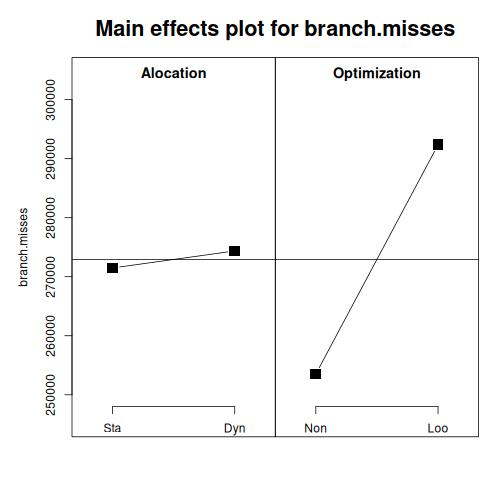
\includegraphics[width=0.6\textwidth]{data/plot/main-effects-bm.jpg}}
\end{center}
\begin{center}
  \makebox[\textwidth]{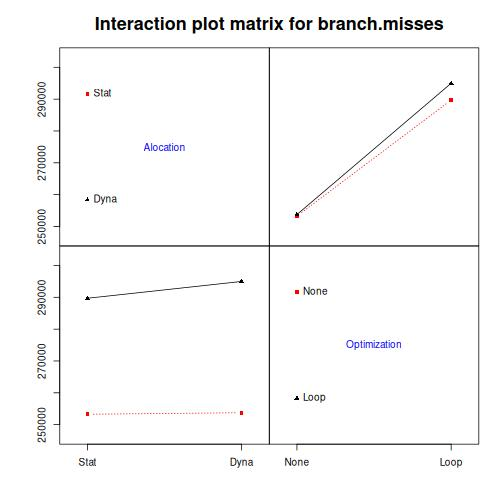
\includegraphics[width=0.6\textwidth]{data/plot/interaction-bm.jpg}}
\end{center}
